\chapter{Électrostatique}
\label{chap:electrostatique}
\label{sec:objectifs}
\begin{objectif}
	\item Connaître les équations qui gouvernent l'évolution spatiale 
	  du champ électrostatique 
	\item Comprendre le lien entre ces équations et une carte de champ 
	  électrique
	\item Déterminer les symétries et invariances d'une distribution de charge
	\item Savoir calculer le champ électrostatique résultant d'une 
	  distribution de charges simple
\end{objectif}
\section*{Introduction}%
\label{sec:introduction}
Les phénomènes électrostatiques sont connus depuis l'Antiquité.
Les Grecs avaient déjà observé que l'ambre (electron en grec)
frottée pouvait attirer des objets
légers comme les copeaux de bois.
Néanmoins, l'étude de ces phénomènes est longtemps restée qualitative.
Il faut attendre le \textsc{xvii} \ieme~siècle pour que des dispositifs 
expérimentaux apparaissent.
Ce premier chapitre s'intéresse à l'étude du champ électrique 
en régime permanent, c'est à dire généré par des charges immobiles dans le 
référentiel d'étude. Les phénomènes décrits dans ce chapitre sont 
donc indépendants du temps.

\begin{defn}{Régime permanent}
	On dit qu'un système fonctionne en régime permanent lorsque toutes les
	grandeurs relatives à une région fixe de ce système sont indépendantes 
	du temps.
\end{defn}

\section{La loi de Coulomb}%
\label{sec:interaction_coulombienne}
En 1785,  le physicien français Charles Augustin de Coulomb (1736-1806)
réalise une étude quantitative de la force d'interaction entre deux particules
chargées à l'aide la balance de Coulomb qu'il a mise au point.
De cette expérience découlent plusieurs observations:

\begin{enumerate}
	\item Il existe deux types de charges: les charges positives et les
	  charges négatives.
	\item Deux charges de même signe se repoussent et deux charges de signes
	  opposés s'attirent.
	\item L'intensité entre les forces est proportionnelle à l'inverse 
	  du carré de la distance qui les sépare.
\end{enumerate}
Ces observations expérimentales se résument dans \emph{la loi de Coulomb}. 


\begin{defn}{Loi de Coulomb}
	La force $\vecf_{1 \rightarrow 2}$ électrostatique
	exercée par une charge $q_1$ située en un point $M_1$ sur une 
	charge $q_2$ située en $M_2$ (voir Fig.~\ref{fig:coulomb}) est donnée par
	\begin{equation}
		\label{eq:loi_coulomb}
		\vecf_{1 \rightarrow 2} = \dfrac{1}{4\pi\epsilon_0}
	                                \dfrac{q_1 q_2}{||M_1M_2||^2}
					\mitbf{e}_{M_1M_2},
	\end{equation}
	où $\epsilon_0 \approx \unit{8.85 \times 10^{-12}}
	{\farad \usk \reciprocal \meter}$ 
	est la permittivité diélectrique
	du vide et $\mitbf{e}_{M_1M_2}$ le vecteur unitaire dirigé de $M_1$ à
	$M_2$. Le farad $\farad$ ($\meter \rpsquared \usk \rp \kilogram
	\usk \second^4 \usk \ampere \squared$ en USI)
	est une unité de capacité électrique.
	Dans la loi de Coulomb,
	\begin{itemize}
		\item la distance s'exprime en mètre,
		\item la charge s'exprime en coulomb noté $\coulomb$
		($\ampere \usk \rp \second$),
		\item la force s'exprime en newton noté $\newton$ 
		  ($\kilogram \usk \meter
		  \usk \rpsquare \second$ dans le système international),
		\item la permittivité diélectrique du vide s'exprime en 
		  $\farad \usk \reciprocal \meter$ 
		  ($\rpcubic \meter \usk \reciprocal \kilogram \usk 
		  \power{\second}{4} \usk \power{\ampere}{2}$ dans le système
		  international).
	\end{itemize}

\end{defn}

\begin{figure}[h!]
	\centering
	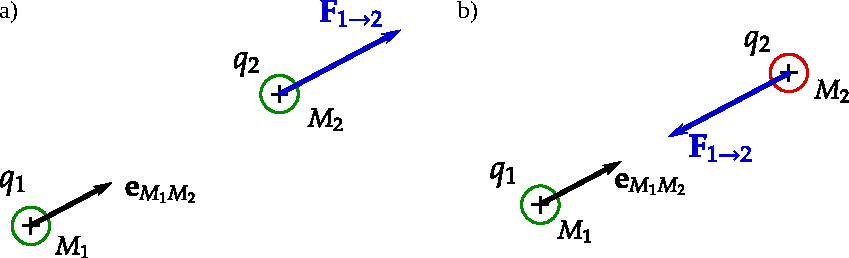
\includegraphics[scale=0.7]{coulomb.pdf}
	\caption{Force exercée par une charge $q_1$ sur une charge $q_2$ dans
	         le cas où les charges sont de même signe (à gauche) et de 
	 	signe opposé (à droite)}%
	\label{fig:coulomb}
\end{figure}


On remarque une forte ressemblance entre cette loi et la loi d'interaction gravitationnelle
proposée par Newton. Nous verrons que cette analogie, résumée par le Tableau~\ref{tab:analogie},
permet d'appliquer des résultats de l'électrostatique à la gravitation et inversement.
Néanmoins, l'interaction électrostatique fait apparaître deux types de charges
électriques et peut donc être soit attractive, soit répulsive. L'
interaction gravitationnelle est quant à elle toujours attractive.

\begin{table}[h!]
	\centering
	\caption{Tableau d'analogie entre force d'interaction électrique et 
	force d'interaction gravitationnelle. $\mathcal{G}$ est la constante 
	universelle de gravitation.}
	\label{tab:analogie}
	\begin{tabular}{c|c}
		Électrostatique 	&	Gravitation \\[1em] \hline \\[0.5em]
		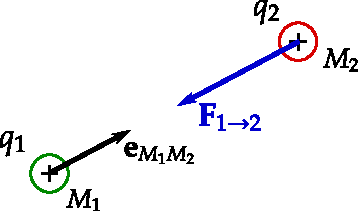
\includegraphics[scale=0.8]{analogie1.pdf} & 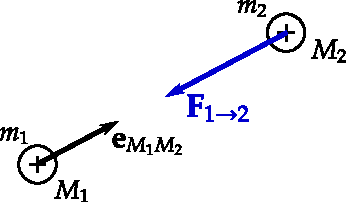
\includegraphics[scale=0.8]{analogie2.pdf} \\[2em]
		$\vecf_{1 \rightarrow 2} = \dfrac{1}{4\pi\epsilon_0}
	                                  \dfrac{q_1 q_2}{||M_1M_2||^2}
					  \mitbf{e}_{M_1M_2}$
					& $\vecf_{1 \rightarrow 2} = - \mathcal{G}
	                                  \dfrac{m_1 m_2}{||M_1M_2||^2}
					  \mitbf{e}_{M_1M_2}$ \\[1em]
		$q_1$			&	$m_1$ \\[1em]
		$\dfrac{1}{4 \pi \epsilon_0}$		&	$-\mathcal{G}$\\
	\end{tabular}
\end{table}

\begin{figure}[h!]
	\centering
	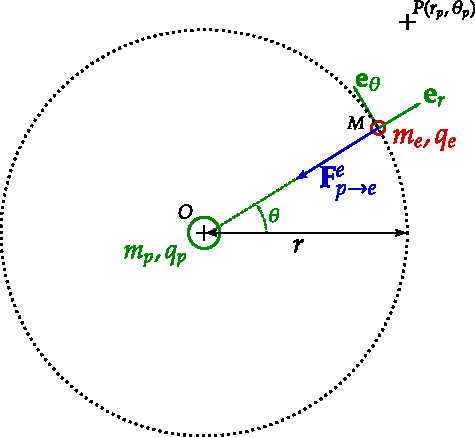
\includegraphics[scale=0.8]{modele_hydrogene}
	\caption{Modèle planétaire de l'atome d'hydrogène. L'électron 
	se trouve sur une orbite circulaire de rayon $r$ en pointillé ici.}%
	\label{fig:hydrogene}
\end{figure}

\begin{exemple}
	\label{ex:hydrogene}
	On considère le modèle planétaire de l'atome d'hydrogène 
	(voir Fig~\ref{fig:hydrogene}).
	Un électron de charge $-e = \unit{-1.60 \times 10^{-19}}{\coulomb}$ et 
	de masse $m_e \approx \unit{9.11 \times 10^{-31}}{\kilogram}$ décrit une
	orbite circulaire de rayon $r = \unit{52.9 \times 10^{-12}}{\meter}$
	autour d'un proton de charge $e$ et de masse
	$m_p \approx \unit{1.67 \times 10^{-27}}{\kilogram}$. 
	Les deux particules s'attirent car leurs charges sont de signe opposé. 
	On cherche à déterminer l'intensité 
	de la force électrostatique $\vecf^e_{p \rightarrow e}$ que le proton 
	exerce sur l'électron.
	La loi de Coulomb~\ref{eq:loi_coulomb} nous donne directement

	\begin{equation*}
		|\vecf^e_{p \rightarrow e}| = \dfrac{1}{4\pi\epsilon_0}
		                         \dfrac{e^2}{r^2}
					\approx \unit{82.7 \times 10^{-9}}{\newton}.
	\end{equation*}

	On peut alors comparer cette valeur à l'intensité de la force 
	d'interaction gravitationnelle
	$\vecf^g_{p \rightarrow e}$ que le proton exerce sur l'électron
	
	\begin{equation*}
		|\vecf^g_{p \rightarrow e}| = \mathcal{G}
		                         \dfrac{m_e m_p}{r^2}
					\approx \unit{36.2 \times 10^{-47}}{\newton},
	\end{equation*}
	avec $\mathcal{G} \approx \unit{6.67 \times 10^{-11}}{\newton \usk 
	\meter \squared \usk \rpsquare \kilogram}$ la constante universelle de
	gravitation. On remarque que l'intensité de la force 
	d'interaction gravitationnelle est bien plus faible que celle de la 
	force électrique, d'environ quarante ordres de grandeur.
	On néglige donc l'interaction gravitationnelle devant l'interaction
	gravitationnelle pour des
	particules chargées.
\end{exemple}


\section{Le champ électrostatique}
L'interaction gravitationnelle et l'interaction électrique ont posé problème aux 
physiciens du \textsc{xvii}\ieme~siècle car il s'agissait d'interaction à distance
sans contact. Faraday a donc introduit la notion de champ afin d'éviter 
ce délicat problème.
En physique, un champ est une fonction qui associe à tout point de l'espace un vecteur,
si le champ est vectoriel, ou un scalaire, si il est scalaire.
La température est par exemple un champ scalaire
et la vitesse est un champ vectoriel.
Une particule chargée exerce alors une force électrostatique sur une autre particule 
par l'intermédiaire du \emph{champ électrostatique} noté $\vece$.

\begin{defn}{Le champ électrostatique}
	Le champ électrostatique $\vece$ créé par une particule de charge $q$
	située au point $M$ de l'espace en un point $P$ est donné par

	\begin{equation}
		\vece(P) = \dfrac{q}{4 \pi \epsilon_0 ||MP||^2}\mitbf{e}_{MP},
	\end{equation}
	où $\mitbf{e}_{MP}$ est le vecteur unitaire dirigé de $M$ vers $P$.
	Le champ électrostatique est un champ vectoriel, à chaque point 
	de l'espace $P$, il associe un vecteur $\vece(P)$.
	Il s'exprime en $\volt \usk \reciprocal \meter$. 
	Connaissant la champ électrique en un point $P$ de l'espace, il est alors
	facile de déterminer la force $\vecf$ que subirait une particule de charge
	$Q$ placée en ce même point

	\begin{equation}
		\vecf = Q\vece(P).
	\end{equation}
\end{defn}

On peut déterminer le champ électrostatique 
créé en un point $P$ par un ensemble de $N$ particules chargées en utilisant
\emph{le principe de superposition}.
En effet, on constate expérimentalement que le champ électrostatique créé par ces
$N$ particules au point $P$ est égal à la somme de tous les champs
électrostatiques créés par toutes les charges.

\begin{defn}{Principe de superposition}
	On considère un ensemble de $N$ particules chargées. Chaque particule $i$
	porte la charge $q_i$ et se trouve en un point $M_i$ de l'espace. Chacune
	d'elle créé en un point $P$ de l'espace un champ électrostatique $\vece_i(P)$.
	Le champ électrostatique total créé au point $P$ est alors donné par 

	\begin{equation}
		\vece(P) = \sum_{i=1}^{N} \vece_i(P)
			 =  \sum_{i=1}^{N} \dfrac{q_i}{4 \pi \epsilon_0 ||M_i P||^2}
			   \mitbf{e}_{M_i P}.
		\label{eq:superposition}
	\end{equation}
	De la même manière, la force $\vecf$ subit par une particule de charge $Q$ 
	située au point $P$ est alors donnée par
	\begin{equation}
		\vecf = Q \vece(P).
	\end{equation}
\end{defn}

\section{Les différentes distributions de charge}
Le plus souvent, la charge électrique est répartie de manière continue dans la 
matière. Dans ce cas, il est alors commode de définir une densité de charge qui
exprimera la quantité de charge contenue dans un volume, dans
une surface ou dans un fil. Chaque petit élément de volume, de surface ou de 
longueur renferme alors une charge notée $\mathrm{d}q$. Pour déterminer le 
champ électrique totale $\vece$ en un point $P$ de l'espace, 
il suffit alors de sommer les petits champs $\mathrm{\textbf{d}}\vece$ créés en $P$ 
par chaque petite charge $\mathrm{d}q$.

\begin{figure}
	\centering
	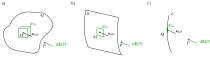
\includegraphics[scale=0.8]{distributions}
	\caption{Illustration de la notion de densité volumique (à gauche),
		 surfacique (milieu) et linéïque (à droite) de charge.}%
	\label{fig:distributions}
\end{figure}

\subsection{Densité volumique de charges}
	On considère une charge $Q$ répartie dans un volume $\mathcal{V}$
	(voir Fig.~\ref{fig:distributions}a). 
	On définit \textbf{
	la densité volumique de charge} $\rho$ 
	telle que pour tout point $M$ du volume,
	la charge $\mathrm{d}q$ contenue dans un petit volume $\mathrm{d}\tau_M$ centré 
	en $M$ est donnée par $\mathrm{d}q = \rho(M) \mathrm{d}\tau_M$.
	Elle s'exprime en $\coulomb \usk \rpcubic \meter$ et vérifie la relation
\begin{equation*}
	\iiint_{M \in \mathcal{V}} \rho(M) \mathrm{d}\tau_M = Q
\end{equation*}
En utilisant le principe de superposition, le champ électrostatique $\vece(P)$
créé au point $P$ de l'espace par une distribution volumique de charge $\rho$
contenue dans un volume $\mathcal{V}$ est
\begin{equation}
	\vece(P) =  \iiint_{M \in \mathcal{V}} 
	\dfrac{\rho(M) \mathrm{d}\tau_M}{4 \pi \epsilon_0 ||MP||^2}\mitbf{e}_{MP},
\end{equation}
où $\dfrac{\rho(M) \mathrm{d}\tau_M}{||MP||^2}\mitbf{e}_{MP}$ est le champ 
électrique créé par le petit volume $\mathrm{d}\tau_M$ au point $P$.

\begin{exemple}
	On considère un noyau d'uranium $238$ de rayon $R = \unit{1}{\femto \meter}$.
	Il contient $92$ protons portant une charge $e$ et $146$ neutrons sans charge.
	On considère que la charge totale $Q$ du noyau est uniformément répartie
	dans le volume du noyau. La densité volumique de charge $\rho$ dans 
	le noyau d'uranium est donc donnée par

	\begin{equation*}
		\rho = \dfrac{Q}{\frac{4}{3}\pi R^3} = 
		\unit{35 \times 10^{27}}{\coulomb \usk \rpcubic \meter}
	\end{equation*}
\end{exemple}

\subsection{Densité surfacique de charge}
	On considère une charge $Q$ répartie sur une surface $\mathcal{S}$
	(voir Fig.~\ref{fig:distributions}b). 
	On définit \emph{
	la densité surfacique de charge} $\sigma$ 
	telle que pour tout point $M$ de la surface,
	la charge $\mathrm{d}q$ contenue sur une petite surface $\mathrm{d}S_M$ centrée 
	en $M$ est donnée par $\mathrm{d}q = \sigma(M) \mathrm{d}S_M$.
	Elle s'exprime en $\coulomb \usk  \meter \rpsquared$ et vérifie la relation
\begin{equation*}
	\iint_{M \in \mathcal{S}} \sigma(M) \mathrm{d}S_M = Q
\end{equation*}
En utilisant le principe de superposition, le champ électrostatique $\vece(P)$
créé au point $P$ de l'espace par une distribution surfacique de charge $\sigma$
contenue sur une surface $\mathcal{S}$ est

\begin{equation}
	\vece(P) = \iint_{M \in \mathcal{S}} 
	\dfrac{\sigma(M) \mathrm{d}S_M}{4 \pi \epsilon_0 ||MP||^2}\mitbf{e}_{MP},
\end{equation}
où $\dfrac{\sigma(M) \mathrm{d}S_M}{||MP||^2}\mitbf{e}_{MP}$ est le champ 
électrique créé par la petite surface $\mathrm{d}S_M$ au point $P$.

\begin{exemple}
	Un condensateur de capacité $C = \unit{1}{\nano \farad}$ est alimenté 
	par une tension $U = \unit{10}{\volt}$. Cette tension induit une 
	accumulation de charges positives et négatives à la surface des deux 
	plaques des surface $S = \unit{2}{\milli \meter \squared}$
	qui le constituent. Une des plaques est alors chargée positivement
	avec la charge $Q = CU = \unit{10^{-8}}{\coulomb}$ 
	tandis que l'autre est chargée négativement avec la 
	charge $-Q$. Si on considère que la charge est uniformément répartie
	sur ces plaques, la densité surfacique de charge de la plaque positive
	est donnée par

	\begin{equation*}
		\sigma = \dfrac{Q}{S} = \unit{5 \times 10^{-3}}
		                        {\coulomb \usk \meter \rpsquared}
	\end{equation*}
\end{exemple}
\subsection{Densité linéïque de charge}
	On considère une charge $Q$ répartie sur un fil $\mathcal{L}$
	(voir Fig.~\ref{fig:distributions}c). 
	On définit \emph{
	la densité linéïque de charge} $\lambda$ 
	telle que pour tout point $M$ du fil,
	la charge $\mathrm{d}q$ contenue sur une petite portion $\mathrm{d}\ell_M$ centrée 
	en $M$ est donnée par $\mathrm{d}q = \lambda(M) \mathrm{d}\ell_M$.
	Elle s'exprime en $\coulomb \usk \reciprocal \meter$ et vérifie la relation
\begin{equation*}
	\int_{M \in \mathcal{L}} \lambda(M) \mathrm{d}\ell_M = Q
\end{equation*}
En utilisant le principe de superposition, le champ électrostatique $\vece(P)$
créé au point $P$ de l'espace par une distribution surfacique de charge $\lambda$
contenue sur un fil $\mathcal{L}$ est

\begin{equation}
	\vece(P) = \int_{M \in \mathcal{L}} 
	\dfrac{\lambda(M) \mathrm{d}\ell_M}{4 \pi \epsilon_0 ||MP||^2}\mitbf{e}_{MP},
\end{equation}
où $\dfrac{\lambda(M) \mathrm{d}\ell_M}{||MP||^2}\mitbf{e}_{MP}$ est le champ 
électrique créé par la petite portion $\mathrm{d}\ell_M$ au point $P$.

\begin{exemple}
	Cette distribution est plus difficile à imaginer.
	On peut par exemple la réaliser en fixant des 
	ions métalliques sur une chaîne de polymères. On considère une chaîne de
	polymère présentant une longueur $L$ de $\unit{1}{\micro \meter}$. On a 
	fixé des ions $Fe^+$ à trois atomes d'intervalle sur cette chaîne.
	La charge est donc répartie de manière uniforme le long du polymère.
	La taille d'un atome étant d'environ $\unit{10^{-10}}{\meter}$, la chaîne de 
	polymère est composée d'environ $10^4$ atomes. Elle porte
	donc une charge totale $Q$ qui vaut $10^4 \times 1.6 \times 10^{-19}/3$.
	On peut alors déduire la
	densité linéïque de charge $\lambda$ de cette chaîne
	\begin{equation}
		\lambda = \dfrac{Q}{L} \approx \dfrac{10^{-6}\times 10^{10}
			           \times 1.6 \times 10^{-19}/3}{10^{-6}}
				= \unit{5.3 \times 10^{-10}}{\coulomb \usk
				   \reciprocal \meter}
	\end{equation}
	où $Q$ est la charge totale fixée sur le polymère.
\end{exemple}

\begin{attention}
	Une distribution volumique de charge est en $\coulomb \usk \rpcubic \meter$,
	une distribution surfacique en $\coulomb \usk \meter \rpsquared$
	et une distribution linéïque en $\coulomb \usk \reciprocal \meter$.
\end{attention}

\section{Équation de l'électrostatique}
On considère une charge ponctuelle $Q$ située à l'origine d'un repère sphérique
$(O, \er, \etheta, \ephi)$ (voir Fig.~\ref{fig:gauss}a). Le champ électrique créé 
par cette charge en 
un point $M(r, \theta, \phi)$ est donné par

\begin{equation*}
	\vece(M) = \dfrac{Q}{4 \pi \epsilon_0 ||OM||^2}\er 
	         = \dfrac{Q}{4\pi\epsilon_0 r^2}\er.
\end{equation*}
Nous allons nous servir de cet exemple simple pour retrouver certaines propriétés
spatiales du champ électrostatique.

\begin{figure}
	\centering
	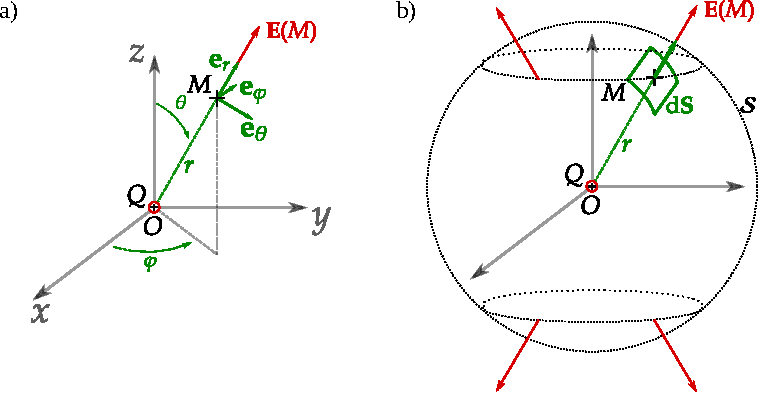
\includegraphics[width=0.8\linewidth]{gauss}
	\caption{Champ créé par une charge ponctuelle $Q > 0$ située en 
		 $O$ au point $M$ (à gauche) et sphère $\mathcal{S}$ à travers
	 	 laquelle on calcule le flux du champ de la charge $Q$ (à droite).
	         $\mathrm{d}\mathbf{S}$ représente un élément infinitésimal 
	 	 de la surface.}%
	\label{fig:gauss}
\end{figure}

\subsection{Le théorème de Gauss}
\label{sec:gauss}
Le théorème de Gauss est un outil puissant qui va nous permettre de calculer
facilement le champ électrique généré par une distribution de charges simple.
Pour le mettre en place, nous
cherchons dans un premier temps à déterminer ``la quantité'' de champ électrique 
$E$ qui traverse une
sphère $\mathcal{S}$ de rayon $r$ centrée en $O$ à laquelle $M$ 
appartient (voir Fig.~\ref{fig:gauss}b). 
La surface $\mathcal{S}$ est ici une surface \emph{fermée}.

\begin{defn}{Surface fermée}
	Une surface est dite fermée si elle délimite un volume intérieur 
	et un volume extérieur. La surface d'une feuille de papier n'est par 
	exemple pas une surface fermée alors que la surface d'un ballon de baudruche
	en est une.
\end{defn}

On commence alors par déterminer 
l'expression du vecteur surface élémentaire $\mathrm{d}\mathbf{S}$. 

\begin{defn}{Vecteur surface élémentaire}
	À chaque élément d'aire $\mathrm{d}S$ centré en $M$ de la surface $\mathcal{S}$, 
	on  affecte un vecteur surface élémentaire $\mathrm{d}\mathbf{S}$ 
	qui vérifie les propriétés suivantes
	\begin{itemize}
		\item il a pour norme l'aire du petit élément de surface centré 
		  au point $M$. Il est donc homogène à une surface.
		\item il est orthogonal à la surface.
		\item il doit être orienté. Cette orientation est au choix de 
		  l'utilisateur.
	\end{itemize}
\end{defn}

\begin{attention}
	Une surface en physique doit toujours être orientée pour savoir
	si le flux qu'on calcule est un flux entrant ou sortant.
\end{attention}

$\mathcal{S}$ est une sphère de rayon $r$ fixé, pour se déplacer à la surface 
de cette dernière, 
il suffit dont de faire varier $\theta$ et $\phi$. $\mathrm{d}\mathbf{S}$ 
étant orthogonal à la surface $\mathcal{S}$, on a

\begin{equation*}
	\ds = r^2 \sin \theta \dtheta \dphi \er.
\end{equation*}
Pour déterminer la quantité de champ électrique qui sort de la surface 
$\mathcal{S}$, on introduit la notion de flux. On retrouve cette notion en géographie,
 où le flux migratoire exprime le nombre de personnes entrant ou sortant d'un 
 pays.

\begin{defn}{Flux d'un champ de vecteurs}
	Soit $M$ un point d'un surface fermée en lequel règne un champ $\vece(M)$.
	Soit $\mathrm{d}\mathbf{S}$ le vecteur surface élémentaire sortant associé
	à l'élément de surface centré en $M$. \emph{Le flux sortant élémentaire} du 
	vecteur $\vece$ à travers $\mathrm{d}S$ est donné par
	$\vece(M) \cdot \mathrm{d}\mathbf{S}$.

	\emph{Le flux total sortant} d'un champ de vecteur $\vece$ à travers 
	une surface fermée
	$\mathcal{S}$ est simplement la somme sur tous les éléments de la surface de tous
	les flux élémentaires sortants
	\begin{equation}
		\oiint_{M \in \mathcal{S}} \vece(M) \cdot \mathrm{d}\mathbf{S}.
	\end{equation}
	Il s'exprime en $\volt \usk \meter$. Le flux est une grandeur algébrique
	qui peut-être positive ou négative. Le symbole $\oiint$ signifie que
	l'intégrale est réalisée sur une surface fermée, il n'est pas obligatoire.
\end{defn}

Le flux de $\vece$ à travers $\mathcal{S}$ s'écrit alors

\begin{equation}
	\oiint_\mathcal{S} \vece \cdot \ds = \oiint_\mathcal{S} \dfrac{Q}{4\pi\epsilon_0 r^2}
	                       r^2 \sin \theta \dtheta \dphi \er \cdot \er
			     = \dfrac{Q}{4 \pi \epsilon_0} \int_0^\pi \sin \theta \dtheta
			     \int_0^{2\pi} \dphi
			     = \dfrac{Q}{\epsilon_0}.
\end{equation}
Ce flux est sortant si la charge $Q$ est positive et est entrant si la charge
$Q$ est négative.
On constate alors que le flux du champ électrique à travers la sphère $\mathcal{S}$
de rayon $r$ ne dépend que de la charge $Q$ qu'elle contient et pas de son rayon.
Cette propriété que nous venons de montrer pour une charge ponctuelle est en 
fait une propriété du champ électrique connue sous le nom de \emph{théorème de 
Gauss}.

\begin{defn}{Théorème de Gauss}
	Le flux du champ électrique $\vece$ à travers une surface fermée $\mathcal{S}$, 
	qui délimite un volume $\mathcal{V}$, est égale à la charge incluse $Q$ dans
	ce volume, divisé par $\epsilon_0$

	\begin{equation}
		\oiint_\mathcal{S} \vece \cdot \ds = \dfrac{Q}{\epsilon_0}.
		\label{eq:gauss}
	\end{equation}
	La surface $S$ est appelée la \emph{surface de Gauss}.
\end{defn}

Le théorème de Gauss peut-être traduit sous une forme locale, 
appelée l'\emph{équation de 
Maxwell-Gauss}, qui relie alors le champ électrique à la distribution de charge.

\begin{defn}{Équation de Maxwell-Gauss}
	L'équation de Maxwell-Gauss relie le champ électrique $\vece$ à la 
	distribution de charge $\rho$

	\begin{equation}
		\div \vece = \dfrac{\rho}{\epsilon_0}.
		\label{eq:MG}
	\end{equation}
	La divergence de $\vece$ est une grandeur scalaire. 
	Cette équation est une relation locale, elle permet de relier
	les dérivées spatiale du champ électrique en un point de l'espace à 
	la densité volumique de charge en ce même point.
\end{defn}

\subsection{Le potentiel électrostatique et l'équation de Maxwell-Faraday}
On cherche maintenant à calculer le rotationnel du champ. 
Cela donne en 
coordonnées sphériques

\begin{equation*}
	\rot \vece = \dfrac{1}{r \sin \theta}\left[\dfrac{1}{r}
		\dfrac{\partial}{\ddtheta}(\sin \theta E_\varphi) - 
	        \dfrac{\partial E_\theta}{\ddphi}\right]\er + 
		\left[\dfrac{1}{r\sin \theta}\dfrac{\partial E_r}{\ddphi} -
		\dfrac{1}{r}\dfrac{\partial}{\ddr}\left(rE_\varphi\right)\right]\etheta
		+ \dfrac{1}{r}\left[\dfrac{\partial}{\ddr}(r E_\theta)
		- \dfrac{\partial E_r}{\ddtheta}\right]\ephi,
\end{equation*}
où $E_r$, $E_\theta$ et $E_\varphi$ sont respectivement les composantes de
$\vece$. Ici, $E_r$ ne dépend que de $r$ et les composantes $E_\theta$ et 
$E_\varphi$ sont nulles. On a donc 

\begin{equation*}
	\rot \vece = \mitbf{0}.
\end{equation*}
Ce résultat se généralise à un champ électrostatique $\vece$ quelconque sous la
forme de l'équation de Maxwell-Faraday.

\begin{defn}{Équation de Maxwell-Faraday}
	Un champ électrique $\vece$ en régime statique, c'est-à-dire
	indépendant du temps, vérifie 
	\begin{equation}
		\rot \vece = \mitbf{0}.
	\end{equation}
	Le rotationnel de $\vece$ est une grandeur vectorielle. Comme
	l'équation de Maxwell-Gauss, l'équation de Maxwell-Faraday est 
	une relation locale vérifiée
	en tout point de l'espace.
\end{defn}

Comme l'équation de Maxwell-Gauss, l'équation de Maxwell-Faraday peut se mettre 
sous une forme intégrale, en exprimant la circulation du champ électrique sur
une courbe fermée $\mathcal{C}$.

\begin{defn}{Circulation d'un champ de vecteurs}
	Soit $\mathbf{W}$ un champ de vecteur et $\mathcal{C}$ un arc de courbe orienté 
	dans l'espace. On appelle circulation du champ de vecteurs $\mathbf{W}$
	le long de $\mathcal{C}$ la quantité
	\begin{equation*}
		\int_{M \in \mathcal{C}} \mathbf{W}(M) \cdot \dl_M.
	\end{equation*}
\end{defn}

\begin{attention}
	Un contour doit toujours être orienté !
\end{attention}

\begin{defn}{Circulation du champ électrostatique}
La circulation du champ électrostatique $\vece$ le long d'un contour fermé
orienté $\mathcal{C}$ est nul
\begin{equation}
	\oint_\mathcal{C} \vece \cdot \dl = 0.
\end{equation}
On dit alors que le champ électrique est à circulation conservative.
\end{defn}

Le champ électrostatique est donc un champ dont le rotationnel est nul en tout 
point de l'espace. L'analyse vectorielle affirme qu'il est possible dans ce cas 
de définir un champ scalaire $V$,
défini à une constante près, 
tel que $\vece = -\gradient V$.

\begin{defn}{Potentiel électrostatique}
	Le champ électrostatique étant à rotationnel nul, il existe un 
	champ scalaire $V$, appelé potentiel électrostatique, tel qu'en
	tout point de l'espace

	\begin{equation}
		\vece = -\gradient V.
		\label{eq:potentiel}
	\end{equation}
	Le potentiel électrostatique s'exprime en volts. Il est toujours défini
	à une constante près.
	La circulation du 
	champ électrostatique entre un point $A$ et un point $B$ est alors donnée
	par

	\begin{equation}
		\int_A^B \vece \cdot \dl = V(A) - V(B)
	\end{equation}
\end{defn}

En reportant $\vece$ par $-\grad V$ dans l'équation de 
Maxwell-Gauss~\ref{eq:MG}, on obtient

\begin{equation*}
	\div(-\grad V) = \dfrac{\rho}{\epsilon_0} \Rightarrow \laplacien V = 
	              -\dfrac{\rho}{\epsilon_0}.
\end{equation*}

\begin{defn}{Équation de Poisson}
	Le potentiel électrique suit l'équation de Poisson
	\begin{equation}
		\laplacien V = -\dfrac{\rho}{\epsilon_0}.
	\end{equation}
\end{defn}

De plus, la force électrostatique est une force conservative. On peut alors
définir une \emph{énergie potentielle} qui lui est associée.

\begin{defn}{Énergie potentielle électrostatique}
	La force électrostatique $\vecf$ est une force conservative, elle 
	dérive donc d'une énergie potentielle $E_p$

	\begin{equation}
		\vecf = - \gradient E_p.
	\end{equation}
	Cette énergie est définie à une constante
	près. Elle s'exprime en joule ($\kilogram \usk \meter \squared \usk \second
	\squared$ en SI). Une charge $q$ placée en un point $M$ de
	l'espace où règne un potentiel électrostatique $V$ possède une 
	énergie potentielle électrostatique 

	\begin{equation*}
		E_p = q V(M) + X,
	\end{equation*}
	où $X$ est une constante. Elle est soumise à la force électrostatique

	\begin{equation*}
		\vecf = -\gradient E_p.
	\end{equation*}
\end{defn}

\begin{exemple}
	Dans l'Exemple~\ref{ex:hydrogene} du modèle planétaire
	de l'atome d'hydrogène, le proton génère
	un potentiel $V$
	\begin{equation*}
		V(r) = \dfrac{e}{4 \pi \epsilon_0 r}.
	\end{equation*}
	L'électron possède donc une énergie potentielle $E_p$ donnée par
	\begin{equation*}
		E_p(r) = -eV(r) = \dfrac{-e^2}{4 \pi \epsilon_0 r} + C,
	\end{equation*}
	où $C$ est une constante. Nous posons $C = 0$, ce qui nous permet d'obtenir une énergie
	potentielle qui est nulle lorsque $r$ tend vers l'infini. L'électron 
	possède alors une énergie potentielle
	$E_p \approx \unit{-27.3}{\electronvolt}$,
        où $\unit{1}{\electronvolt} \approx \unit{1.60 \times 10^{-19}}{\joule}$.
	L'application du principe fondamental de la dynamique à l'électron permet
	de déterminer la vitesse de ce dernier dans le référentiel d'étude.
	On peut alors en déduire son énergie cinétique
	\begin{equation*}
		E_c = \dfrac{e^2}{8 \pi \epsilon_0 r} = \unit{13.7}{\electronvolt}.
	\end{equation*}
	Finalement, l'électron possède une énergie totale de $-\unit{13.6}{\electronvolt}$.
\end{exemple}

\section{Étude des lignes de champ de \vece}
Nous nous intéressons dans cette partie aux propriétés spatiales du champ $\vece$.
Nous allons voir comment les \emph{lignes de champ} nous renseignent sur sa répartition 
dans l'espace.

\begin{defn}{Ligne de champ}
	Une ligne de champ est une courbe tangente en chaque point au vecteur 
	du champ de vecteurs considéré, orientée dans le sens du champ. Deux
	lignes de champ ne peuvent pas se croiser.
\end{defn}

Pour déterminer l'équation de ces lignes de champ, il suffit de résoudre l'équation
qui traduit la tangence en tout point de l'espace $M$ des lignes de champ 
au vecteur $\vece(M$)

\begin{equation}
	\vece \times \dl = \mitbf{0},
\end{equation}
où $\dl$ est un élément de la ligne de champ.



\begin{exemple}
	Les lignes du champ électrostatique $\vece$ généré par une charge ponctuelle $q$
	sont des droites portées par un rayon de la charge (voir Fig~\ref{fig:lignes}). 
	Si la charge est positive, elles sont orientées vers l'extérieur. À
	l'inverse si elle
	est négative, elles sont orientés vers la charge. On cherche à déterminer l'équation
	de ces lignes de champ. On se place dans un repère sphérique $(\er, \etheta, \ephi)$
	centré sur le centre de la charge $q$. Un point de l'espace $M$ est donc repéré par
	ses coordonnées $(r, \theta, \varphi)$. Un élément $\dl$ de la ligne de champ 
	passant par $M$ doit vérifier
	\begin{equation*}
		\vece(M) \times \dl = \mitbf{0} \Rightarrow
		\dfrac{q}{4 \pi \epsilon_0}
		\begin{array}{|l}
			1/r^2 \\[1em]
			0 \\[1em]
		0 \\
		\end{array}
		\times
		\begin{array}{|l}
			\dr \\[1em] 
			r \dtheta \\[1em]
			r \sin \theta \dphi \\
		\end{array}
		= \mitbf{0}
		\Rightarrow
		\begin{array}{|l}
			0 \\[1em] 
			\sin \theta \dphi/r \\[1em]
			\dtheta/r \\
		\end{array}
		= \mitbf{0}
		\Rightarrow
		\left\{
		\begin{array}{rcl}
			\sin \theta \dphi/r = 0 \\[1em]
			\dtheta/r = 0 \\
		\end{array}
		\right.
	\end{equation*}
En d'autres termes, tous les points de cette ligne de champ doivent avoir le 
même $\theta$ et le même $\varphi$. Les lignes de champ sont donc bien portées 
par des rayons de la charge.
\end{exemple}

\begin{figure}[h!]
	\centering
	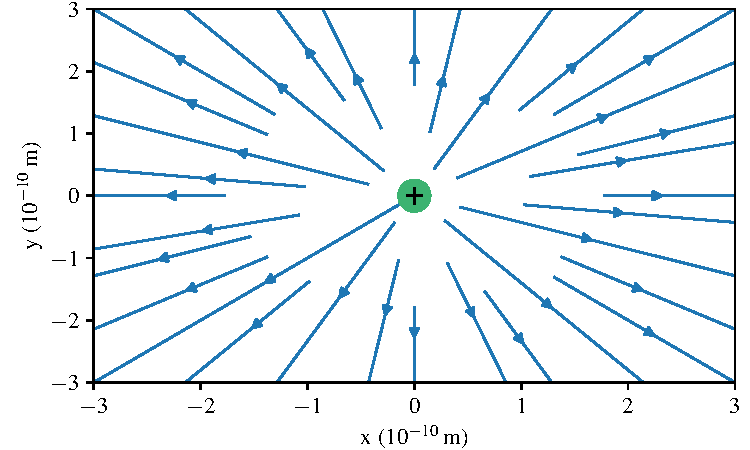
\includegraphics[width=0.45\linewidth]{charge+}
	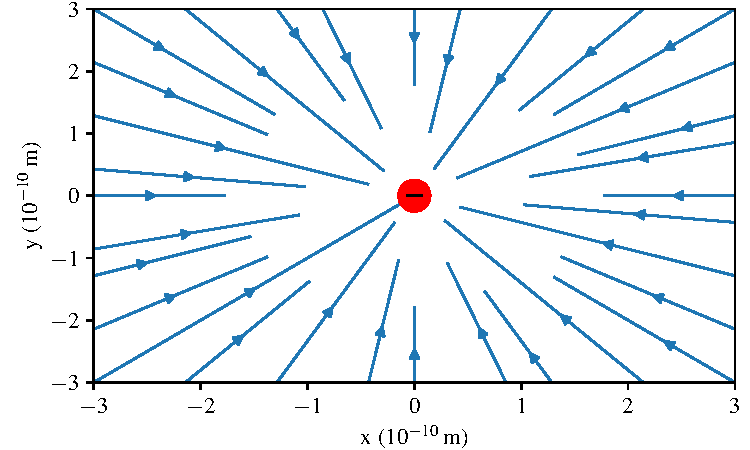
\includegraphics[width=0.45\linewidth]{charge-}
	\caption{Ligne du champ $\vece$ créé par une charge positive (à gauche)
	         et par une charge négative (à droite).}%
	\label{fig:lignes}
\end{figure}

Nous allons maintenant considérer la cas d'un proton et d'un électron séparé 
par une distance de $\unit{0.2}{\nano \meter}$ (voir Fig.~\ref{fig:dipole}).
Les lignes de champ nous permettent de retrouver quelques propriétés du champ 
électrostatique énoncées précédemment.

\begin{figure}[h!]
	\centering
	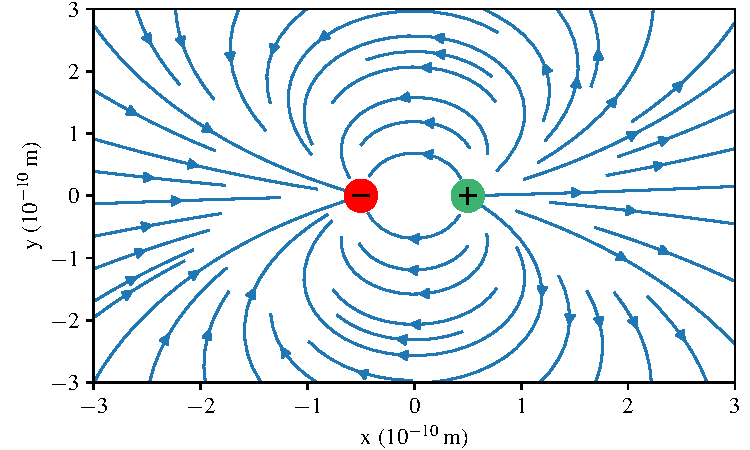
\includegraphics[scale=0.75]{dipole}
	\caption{Lignes du champ électrique généré par un proton (charge verte) et 
	         un électron (charge rouge).}%
	\label{fig:dipole}
\end{figure}

\begin{enumerate}
	\item On remarque tout d'abord que les lignes de champ sont orientées 
	  de la charge positive vers la charge négative. Cette première 
	  observation peut être vue comme une conséquence de la relation reliant 
	  le champ électrique $\vece$ et le potentiel électrostatique $V$ 
	  (voir Eq.~\ref{eq:potentiel}). En effet, le sens de $\vece$ est 
	  opposé à celui du gradient de $V$ (comme le traduit le signe $-$ dans 
	  l'expression).
	  La ligne de champ s'écoule donc du potentiel le plus élevé 
	  vers le moins élevé.
      \item La divergence d'un champ vectoriel permet de mesurer
	    le flux de ce dernier à travers un volume. Si elle est nulle, 
	    une ligne de champ entrant dans un volume doit absolument en ressortir.
	    La divergence non nulle du champ électrique (voir Eq.~\ref{eq:MG})
	    se traduit par la possibilité pour les lignes de champ d'émerger d'un 
	    volume (du proton ici) et de converger dans un volume (l'électron ici).

	    \item Le rotationnel d'un champ vectoriel traduit la tendance de ce dernier
	    à tourner autour d'un point.
	    Le rotationnel nul du champ électrique se traduit par l'impossibilité
	    pour les lignes de champ de tourner autour d'un point. Une ligne du champ
	    électrique ne peut donc pas reboucler sur elle-même.

    	   \item Grâce aux lignes de champ, on retrouve rapidement les plans de 
		 symétrie et d'antisymétrie du champ électrique. Le plan médiateur 
		 est par exemple un plan d'antisymétrie du champ électrique. 
		 L'analyse de ces symétries sera utile pour calculer le champ
		 électrique d'une distribution de charge.
\end{enumerate}

\section{Calcul du champ électrostatique}
\label{sec:calcul_e}
Nous allons voir dans cette partie comment nous pouvons utiliser le théorème de
Gauss pour calculer le champ électrique créé 
par une distribution de charges simple. Nous nous intéressons ici à une boule de
rayon $R_1$ et de centre $O_1$ uniformément chargée avec une densité volumique
de charge $\rho > 0$ (voir Fig.~\ref{fig:cavite1}). On cherche à déterminer 
l'expression du champ électrique $\vece$ en un point $M$ de l'espace. Pour ce faire, 
il suffit de suivre le mode d'emploi suivant
\begin{enumerate}
	\item Faire un schéma du système ! C'est absolument indispensable
	  (voir Fig.~\ref{fig:cavite1})
	\item Choisir un repère adapté au problème
	\item Étudier les invariances de cette distribution
	\item Étudier les symétries de la distribution de charges à l'origine 
	  du champ électrique
	\item Choisir une surface de Gauss et appliquer le théorème de Gauss.
\end{enumerate}

Nous choisissons ici d'utiliser un repère sphérique $(O_1, \er, \etheta, \ephi)$.
Le point $M$ est donc repéré par ses coordonnées $(r, \theta, \phi)$. Le champ
électrique en $M$ s'écrit de manière générale

\begin{equation}
	\vece(M) = E_r(M)\er + E_\theta(M)\etheta + E_\varphi(M)\ephi.
	\label{eq:cavite1}
\end{equation}
Le champ électrique est un vecteur à trois composantes et chaque composante
dépend des coordonnées de $M$. Pour simplifier cette expression, il est intéressant
de considérer les invariances et symétries de la distribution de charge qui génère
le champ $\vece$.

\begin{figure}
	\centering
	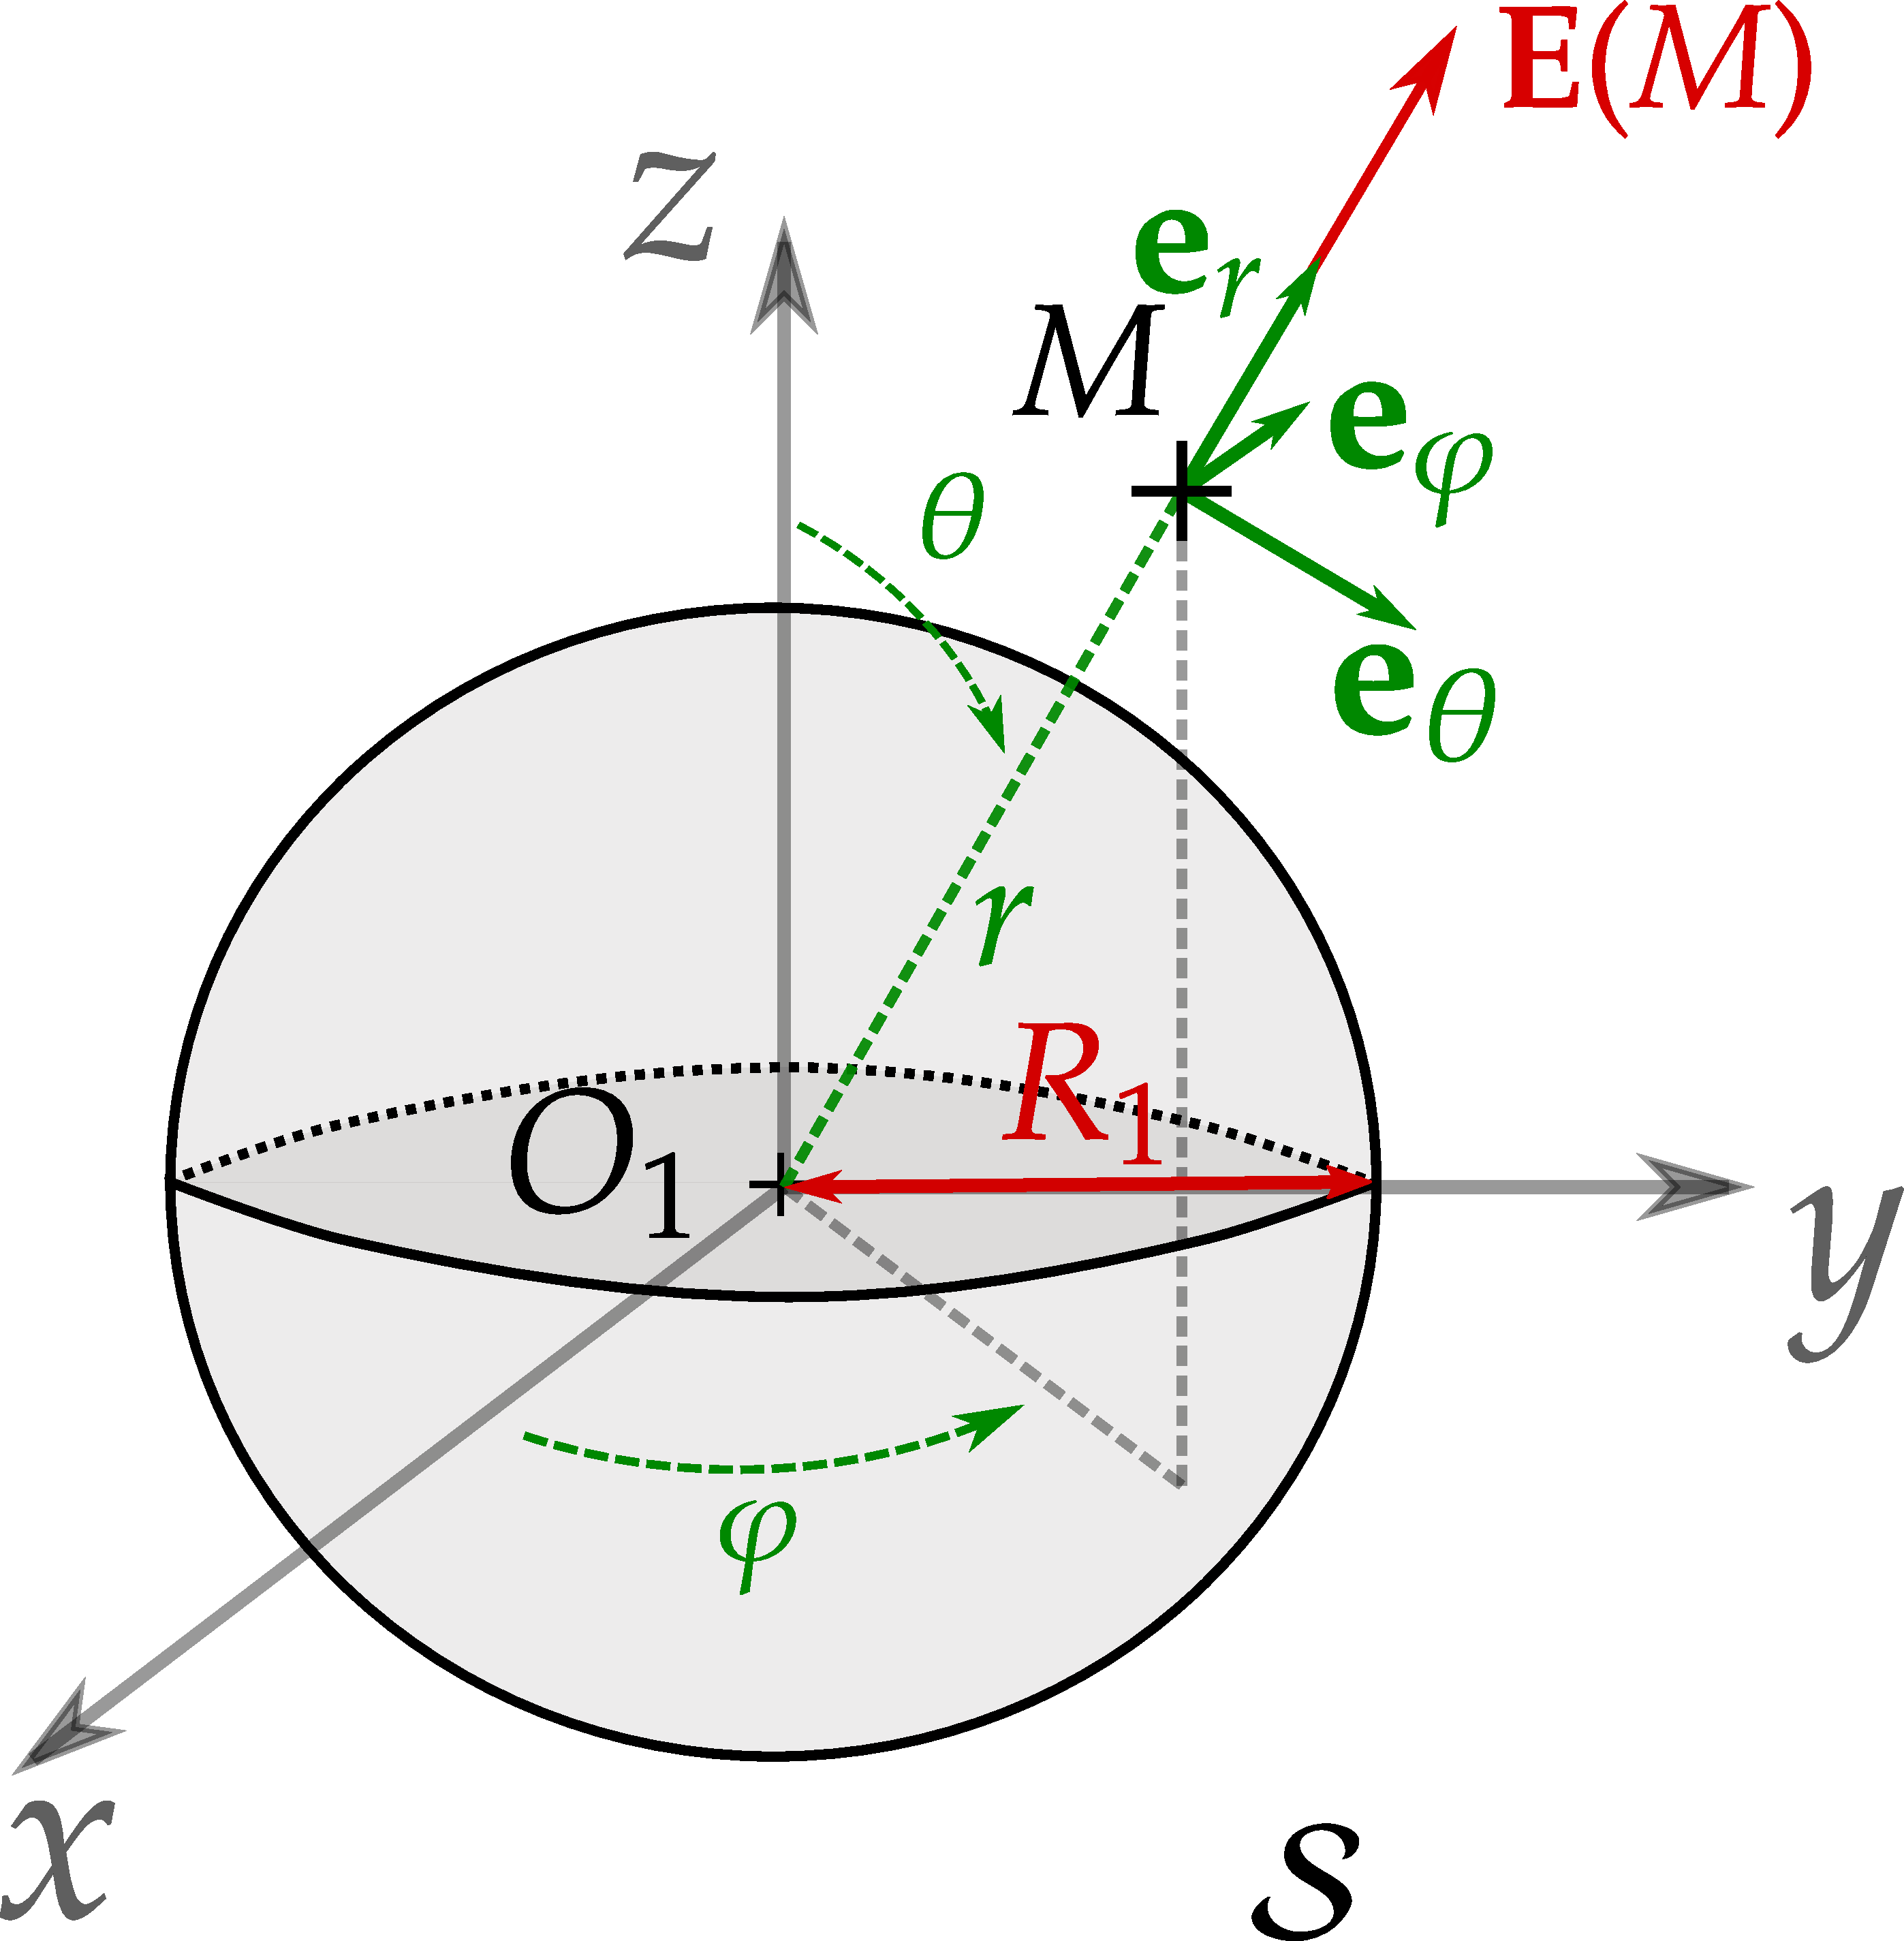
\includegraphics[scale=1]{cavite1}
	\caption{Schéma de la cavité uniformément chargée.}%
	\label{fig:cavite1}
\end{figure}

\subsection{Invariance de la distribution de charges}
On cherche ici à savoir si la distribution de charge est modifiée sous l'effet
d'une translation ou d'une rotation de l'espace. En d'autres termes, on regarde
de quelles variables dépend la densité de charge $\rho$. Étant donné que la
sphère est ici uniformément chargée, on observe que

\begin{itemize}
	\item  si je tourne la sphère d'un angle $\Delta \theta$ dans la
	  direction $\etheta$, le problème
	  ne change pas. La distribution de charge est donc invariante 
	  par rotation selon l'angle $\theta$. $\vece$ ne dépend pas de
	  $\mitbf{\theta}$.

	  \item  si je tourne la sphère d'un angle $\Delta \varphi$ dans la
	  direction $\ephi$, le problème
	  ne change pas. La distribution de charge est donc invariante 
	  par rotation selon l'angle $\varphi$. $\vece$ ne dépend pas de
	  $\mitbf{\varphi}$.
  	\item si je déplace la sphère d'une distance $\Delta r$ dans la direction
	$\er$ je remarque que le problème change. Par exemple si $\Delta r$ 
	est supérieur à $R_1$, le point $O_1$ n'appartient plus à la sphère après
	la translation. $\vece$ dépend de $\mitbf{r}$.

\end{itemize}

Finalement, l'expression~\ref{eq:cavite1} du champ électrique se simplifie

\begin{equation}
	\vece(M) = E_r(r)\er + E_\theta(r)\etheta + E_\varphi(r)\ephi.
\end{equation}
\subsection{Symétries de la distribution de charges}

\begin{defn}{Principe de Curie}
	Lorsque les causes produisent des effets, les symétries présentes dans les
	causes doivent se retrouver dans celles des effets.
\end{defn}

Si on applique ce principe au champ électrique créé par une distribution 
de charges, cela revient à dire que les symétries de la distribution de 
charges doivent se retrouver dans les symétries du champ électrique. On en 
déduit les règles suivantes

\begin{defn}{Symétries de $\vece$ et de la distribution de charge}
  \begin{itemize}
  \item si $(\Pi)$ est un plan de symétrie de la distribution de charge et que 
    $M$ appartient à $(\Pi)$, alors obligatoirement $\vece(M)$ doit 
    appartenir à $(\Pi)$,
  \item si $(\Pi)$ est un plan d'antisymétrie de la distribution de charge 
    et que $M$ appartient à $(\Pi)$, alors obligatoirement $\vece(M)$ doit 
    être orthogonal à $(\Pi)$.
  \end{itemize}
\end{defn}

Pour appliquer ces règles à notre exemple, on détermine les plans de symétrie 
et d'antisymétrie de la distribution de charges auxquels 
le point $M$ appartient

\begin{itemize}
	\item le plan $(M, \er, \etheta)$ est un plan de symétrie de la distribution
		de charge. $\vece(M)$ doit donc appartenir à ce plan.
        \item le plan $(M, \er, \ephi)$ est un plan de symétrie de la distribution de 
		charge. $\vece(M)$ doit donc appartenir à ce plan.
\end{itemize}

$\vece(M)$ doit appartenir au plan $(M, \er, \etheta)$ et au plan $(M, \er, \ephi)$.
$\vece$ doit donc être colinéaire à $\er$

\begin{equation}
	\vece(M) = E_r(r) \er.
\end{equation}
Nous n'avons imposé aucune condition sur la position de $M$, cette relation est
donc vraie pour tout point $M$ de l'espace. Maintenant que l'expression du 
champ électrique a été simplifiée au maximum, on cherche à appliquer le théorème
de Gauss.

\subsection{Application du théorème de Gauss}
\begin{figure}
	\centering
	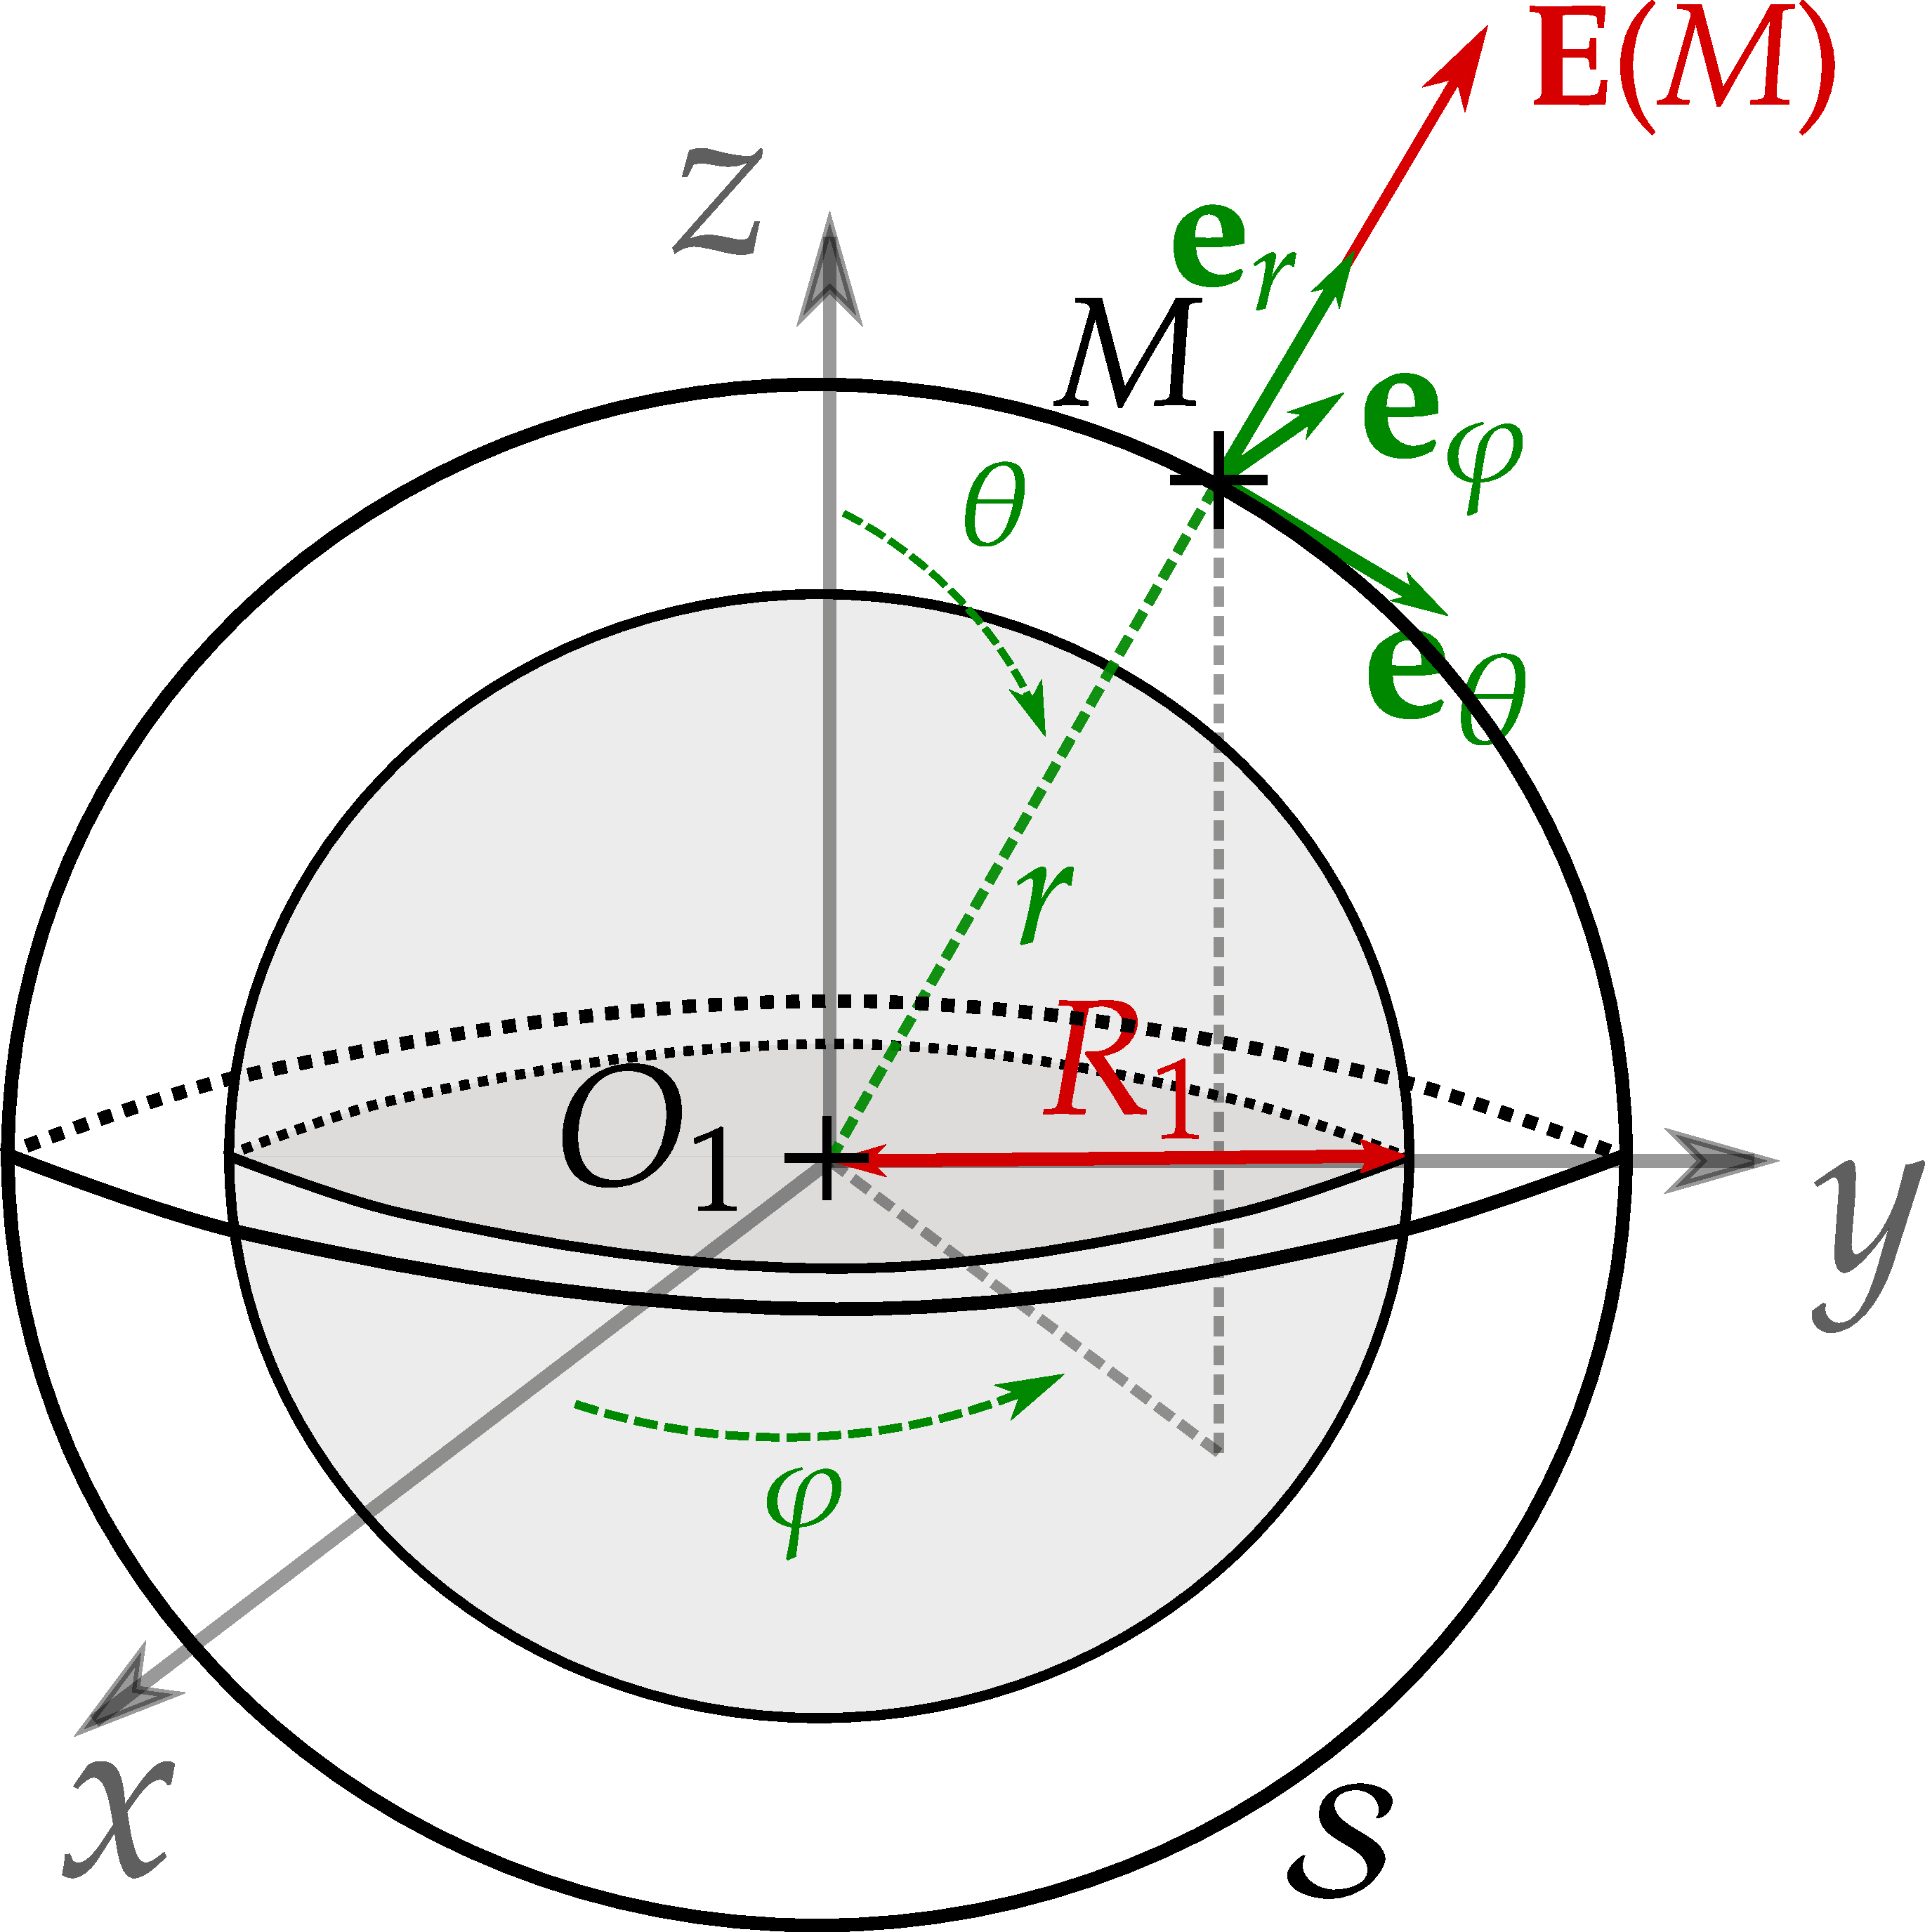
\includegraphics[scale=1]{cavite1_gauss}
	\caption{Schéma de la cavité avec la surface de Gauss $\mathcal{S}$
	         qui est une sphère de rayon $r$ et de centre $O_1$. $M$
	         appartient à cette surface.}%
	\label{fig:cavite_gauss}
\end{figure}

La distribution de charge présente une symétrie sphérique. On choisit comme surface 
de Gauss une sphère de rayon $r$ et de centre $O_1$ 
(voir Fig~\ref{fig:cavite_gauss}) et on applique le théorème de Gauss sur cette
sphère

\begin{equation}
	\oiint_\mathcal{S} \vece(M) \cdot \ds = \dfrac{Q}{\epsilon_0},
	\label{eq:cavite_gauss}
\end{equation}
où $Q$ est la charge contenue à l'intérieur de $\mathcal{S}$. On commence
par déterminer l'expression du membre de gauche. Comme nous l'avons vu 
(voir Sec.~\ref{sec:gauss}), dans le cas d'une sphère,

\begin{equation}
	\ds = r^2 \sin \theta \dtheta \dphi \er.
\end{equation}
On obtient alors
\begin{equation}
	\oiint_\mathcal{S} \vece(M) \cdot \ds = 
	\oiint_\mathcal{S} E(r) \er \cdot r^2 \sin \theta \dtheta \dphi \er
	= E(r) r^2 \int_0^{2 \pi} \dphi \int_0^\pi\sin \theta \dtheta
	= 4 \pi E(r) r^2.
\end{equation}
On s'intéresse maintenant au terme de droite de l'équation~\ref{eq:cavite_gauss}.
La charge $Q$ est uniformément répartie dans la sphère de rayon $R_1$, on a donc

\begin{equation}
	\rho(r) = 
	\left\{
	\begin{array}{l}
		0,\ \mathrm{si} \  r > R_1,\\[1em]
		\dfrac{Q}{\dfrac{4}{3} \pi r^3},\ \mathrm{si} \ r \leq R_1. \\
	\end{array}
	\right.
\end{equation}
On a alors deux cas de figure
\begin{enumerate}
	\item si $r \leq R_1$, $Q = \dfrac{4}{3 \epsilon_0} \pi r^3 \rho$
	  $\Rightarrow \vece(r) = \dfrac{\rho r}{3 \epsilon_0} \er$.
	\item si $r > R_1$, $Q = \dfrac{4}{3} \pi R_1^3 \rho$ 
	  $\Rightarrow \vece(r) = \dfrac{\rho R_1^3}{3 \epsilon_0 r^2} \er$.
\end{enumerate}

\begin{rema}
	Si on remplace $\rho$ par son expression en fonction de $Q$, 
	$\rho = \dfrac{3Q}{4 \pi R_1^3}$, dans la deuxième 
	situation, on retrouve le champ électrique généré par une charge ponctuelle.
\end{rema}
